\newpage
\setcounter{table}{0}
\setcounter{figure}{0}
\setcounter{section}{0}
\renewcommand\thesection{A.\arabic{section}} 
\renewcommand\thefigure{A\arabic{figure}} 
\renewcommand\thetable{A\arabic{table}} 
\fancyfoot[RO,LE]{APPENDICES}

\chapter*{Appendices}
\addcontentsline{toc}{chapter}{Appendices}

\section{Cancers of interest and putative original cells}
\begin{table}[hp!]
\centering
\caption{\textbf{12 cancers of interest, their abbreviation and their putative original cell types.} The \textbf{Cell line code} column is the code for DHS data of the original cell type, set by the ENCODE project; \textbf{Source} cites the publication that establishes the relationship between the cancer and the original tissue.}
\label{tab:encode}
\begin{tabulary}{\textwidth}{ LlLLR }
\toprule
\bf{Cancer Type} & \bf{Abbreviation} & \bf{Tissue of origin} & \textbf{Cell line code} & \bf{Source} \\
\toprule
Osteosarcoma & Bone-Osteosarc & Connective cells of the bone & Osteobl & \citet{Alfranca2015BoneDevelopment} \\ \hline

Breast Adenocarcinoma & Breast-AdenoCa & Breast epithelium & HMEC & \citet{Boyce2007BreastCancer} \\ \hline

Medulloblastoma &  CNS-Medullo &  Cerebellum & Cerebellum\_OC & \citet{Penas2015TheMedulloblastoma} \\ \hline

Pilocytic Astrocytoma & CNS-PiloAstro & Astrocytes & HAc & \citet{Collins2015PilocyticMarkers}\\ \hline

Kidney Rectal Cell Carcinoma & Kidney-RCC & Renal proximal tubule epithelium & REPTEC & \citet{Hsieh2017RenalCarcinoma} \\ \hline

Liver Hepatocellular Carcinoma & Liver-HCC & Hepatocytes & Hepatocytes & \citet{Gissen2015StructuralDisease} \\ \hline

B Cell Non-Hodgekin Lymphoma & Lymph-BNHL & B cells & B cells CD20+ RO01794 & \citet{Shankland2012Non-HodgkinLymphoma} \\ \hline

Chronic Lymphocytic Leukemia & Lymph-CLL & B cells & B cells CD20+ RO01794 & \citet{Hallek2018ChronicLeukaemia} \\ \hline

Pancreatic Andenocarcinoma & Panc-AdenoCa & Exocrine cells & HPDE6-E6E7 & \citet{Vareedayah2018PancreaticAdenocarcinoma} \\ \hline

Pancreatic Endocrine Cancer & Panc-Endocrine & Islet cells & PanIslets & \citet{Nakakura2007IsletRegion} \\ \hline

Prostate Adenocarcinoma & Prost-AdenoCa & Prostate epithelium & RWPE1 & \citet{Lee2011OverviewPathology} \\ \hline

Skin Melanoma & Skin-Melanoma & Melanocytes &  Melano & \cite{Lin2007MelanocytePigmentation} \\
\bottomrule

\end{tabulary}
\end{table}

% . DHS data for these cells is downloaded from either \href{https://genome.ucsc.edu/cgi-bin/hgFileUi?db=hg19&g=wgEncodeOpenChromDnase}{Duke} or \href{https://genome.ucsc.edu/cgi-bin/hgFileUi?db=hg19&g=wgEncodeUwDnase}{UW} project

\section{PCAWG mutation summary}
\vspace{1cm}
\begin{table}[hp!]
\centering
\caption{Mutation summary for loop 1}
\label{tab:mutation_summary}
\begin{tabulary}{\textwidth}{ rRRRR }
\hline
\bf{Cancer Type} & \bf{Number of donors} & \bf{Average number of mutations} & \bf{Total number of mutations} & \bf{Standard deviation of mutations} \\
\hline
  Bone-Osteosarc &               44 &                   3792 &                    166845 &                       3003.40 \\
  Breast-AdenoCa &              113 &                   6318 &                    713855 &                       8610.10 \\
     CNS-Medullo &              146 &                   1438 &                    209997 &                       1053.20 \\
   CNS-PiloAstro &               89 &                    247 &                     22020 &                        220.70 \\
      Kidney-RCC &               74 &                   7188 &                    531886 &                       5774.70 \\
       Liver-HCC &              264 &                  12582 &                   3321521 &                       6731.50 \\
      Lymph-BNHL &               98 &                  11478 &                   1124881 &                      14534.10 \\
       Lymph-CLL &               95 &                   2381 &                    226242 &                        889.60 \\
    Panc-AdenoCA &              239 &                   7012 &                   1675781 &                       8041.50 \\
  Panc-Endocrine &               85 &                   3042 &                    258564 &                       3284.80 \\
   Prost-AdenoCA &              191 &                   5238 &                   1000496 &                       8892.70 \\
   Skin-Melanoma &               70 &                 111014 &                   7770980 &                     145095.00 \\
\hline
\end{tabulary}
\end{table}

\vspace{2cm}
\begin{figure}[h!]
    \centering
    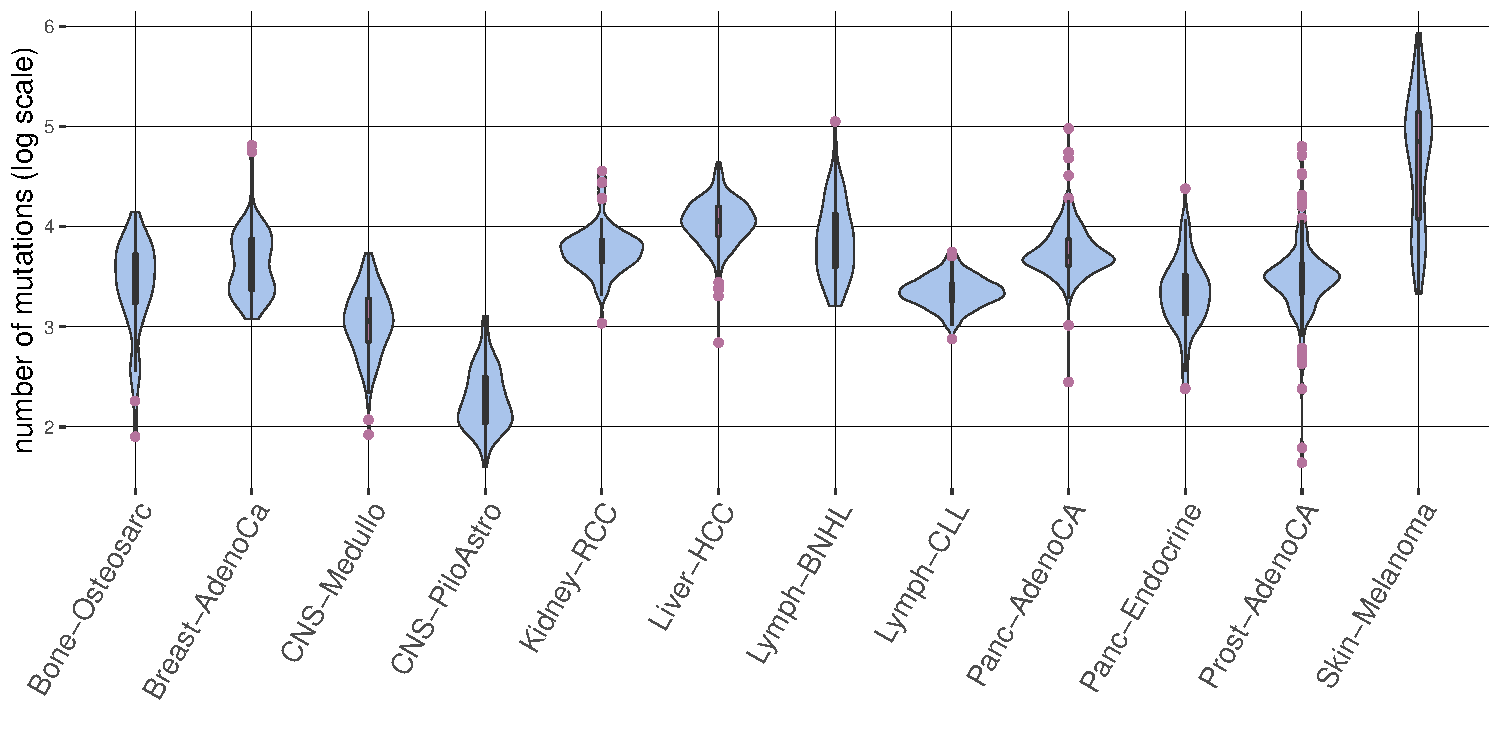
\includegraphics[scale=0.66]{graphics/mutation_summary.pdf}
    \caption{\textbf{Number of mutations (log scale) for each cancer.} Each dot represents a donor. Most patients have approximately 1000-10000 mutations, but there is a great variation.}
    \label{fig:mutation_summary}
\end{figure}


\newpage
\section{How cancer original cell types are related by DHS}
% \begin{figure}[h!]
%     \begin{subfigure}{.5\textwidth}
%     \centering
%     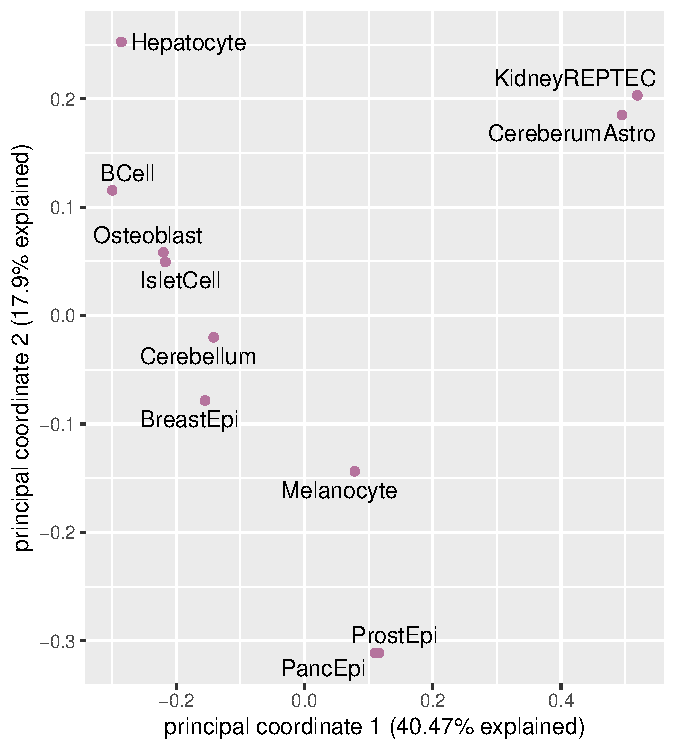
\includegraphics[scale=0.7]{graphics/encode_pca_1_2.pdf}
%     \caption{PC2 \textit{v.s.} PC1}
%     \end{subfigure}
%     ~
%     \begin{subfigure}{.5\textwidth}
%     \centering
%     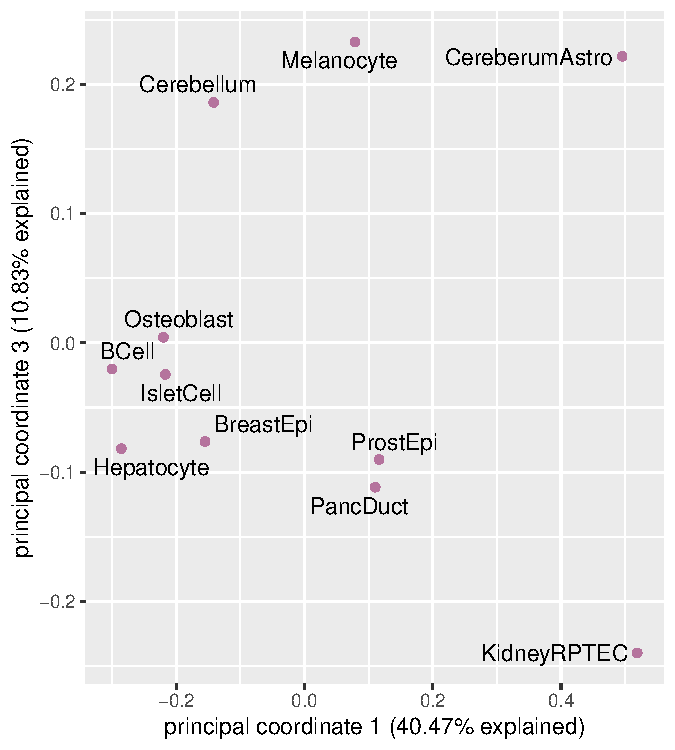
\includegraphics[scale=0.7]{graphics/encode_pca_1_3.pdf}
%     \caption{PC3 \textit{v.s.} PC1}
%     \end{subfigure} \\
%     \caption{\textbf{PCA}.}
%     \label{fig:encode_pca}
% \end{figure}

\begin{figure}[h!]
  \begin{minipage}[c]{\textwidth}
    \begin{subfigure}{.5\textwidth}
    \centering
    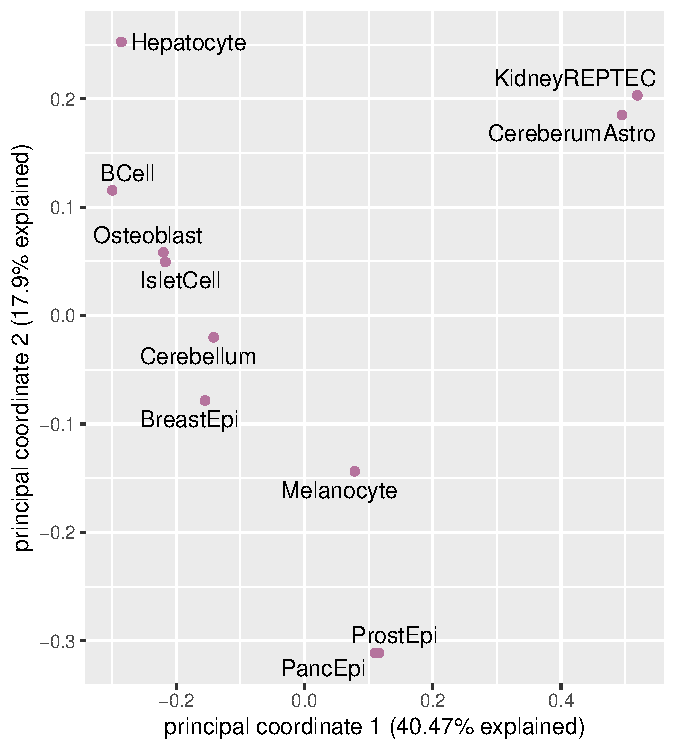
\includegraphics[scale=0.7]{graphics/encode_pca_1_2.pdf}
    \caption{PC2 \textit{v.s.} PC1}
    \end{subfigure}
    ~
    \begin{subfigure}{.5\textwidth}
    \centering
    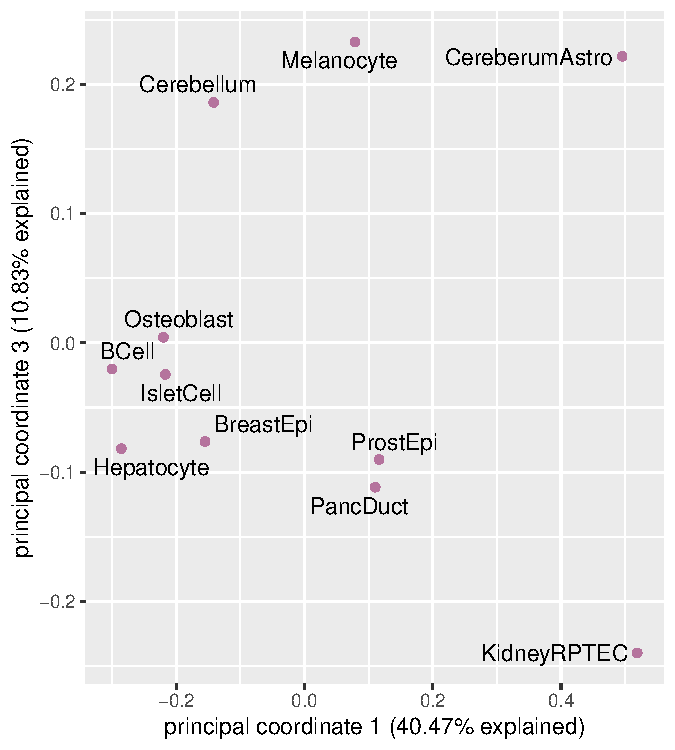
\includegraphics[scale=0.7]{graphics/encode_pca_1_3.pdf}
    \caption{PC3 \textit{v.s.} PC1}
    \end{subfigure} \\
  \end{minipage}\hfill
  \vspace{1cm}
  
  \begin{minipage}[c]{\textwidth}
    \centering
    \begin{tabulary}{\textwidth}{ ll }
    \toprule
    \textbf{Original cell abbreviation} & \bf{Cancer Type}  \\
    \toprule
    Osteoblast & Osteosarcoma \\
    
    BreastEpi & Breast-AdenoCa \\
    
    Cerebellum &  CNS-Medullo  \\
    
    CereberumAstro & CNS-PiloAstro \\
    
    KidneyRPTEC & Kidney-RCC \\
    
    Hepatocyte & Liver-HCC \\
    
    BCell & Lymph-BNHL, Lymph-CLL \\
    
    PancDuct & Panc-AdenoCa \\
    
    IsletCell & Panc-Endocrine \\
    
    ProstEpi & Prost-AdenoCa \\
    
    Melanocyte & Skin-Melanoma \\
    \bottomrule
    
    \end{tabulary}
    
    % . DHS data for these cells is downloaded from either \href{https://genome.ucsc.edu/cgi-bin/hgFileUi?db=hg19&g=wgEncodeOpenChromDnase}{Duke} or \href{https://genome.ucsc.edu/cgi-bin/hgFileUi?db=hg19&g=wgEncodeUwDnase}{UW} project
  \end{minipage}\hfill
  \vspace{0.5cm}
  
  \begin{minipage}[c]{\textwidth}
    \caption{
      \textbf{Some cancers were more related in terms of chromatin structures than others.} Here, I visualised the relative coordinates of the original cell types for cancers on the most informative dimensions (principle coordinates, PC). This was done by multidimensional scaling of the pairwise distance between cell types. The distance between two cell types was computed based on the intersection between their open chromatin regions. 
    } \label{fig:encode_pca}
  \end{minipage}
\end{figure}

\vspace{1cm}
\begin{table}[hp!]
\centering
\caption{\textbf{12 cancers of interest, their abbreviation and their putative original cell types.} The \textbf{Cell line code} column is the code for DHS data of the original cell type, set by the ENCODE project; \textbf{Source} cites the publication that establishes the relationship between the cancer and the original tissue.}
\label{tab:encode_pca}
\begin{tabulary}{\textwidth}{ ll }
\toprule
\textbf{Original cell type} & \bf{Cancer Type}  \\
\toprule
Osteoblast & Osteosarcoma \\

BreastEpi & Breast-AdenoCa \\

Cerebellum &  CNS-Medullo  \\

CereberumAstro & CNS-PiloAstro \\

KidneyREPTEC & Kidney-RCC \\

Hepatocyte & Liver-HCC \\

BCell & Lymph-BNHL \\

BCell & Lymph-CLL \\

PancEpi & Panc-AdenoCa \\

IsletCell & Panc-Endocrine \\

ProstEpi & Prost-AdenoCa \\

Melanocyte & Skin-Melanoma \\
\bottomrule

\end{tabulary}
\end{table}

% . DHS data for these cells is downloaded from either \href{https://genome.ucsc.edu/cgi-bin/hgFileUi?db=hg19&g=wgEncodeOpenChromDnase}{Duke} or \href{https://genome.ucsc.edu/cgi-bin/hgFileUi?db=hg19&g=wgEncodeUwDnase}{UW} project

\newpage
\section{Supplementary computations for smoothing GLE}
\subsection{Gaussian kernel density estimation}

Kernel functions estimate the density of data at a particular location by measuring the distance from that location to all observed data points. To estimate mutation density across the genome, I used the Gaussian kernel, as follows:

\begin{equation}
    K(u) = \frac{1}{2\pi} e^{\frac{-u^2}{2}}
    \label{eq:gaussian}
\end{equation}

where $K$ is the kernel function, $u$ is a variable - \textit{i.e.} $\frac{x-X{i}}{h}$ in equation \ref{eq:density}

\subsection{Bandwidth choice}
The bandwidth $h$ determines the level of smoothing, or the distance at which the an observed mutation can meaningfully influence the density $\hat{f}$ at location $x$, I used the Scott's method, as follows:

\begin{equation}
    h = 1.059 A n^{-1/5}
    \label{eq:bandwidth}
\end{equation}

where $h$ is the bandwidth, $A$ is a measure of spread of the observed mutation locations (\textit{i.e.} the smaller of (1) the standard deviation and the (2) inter-quartile range) and $n$ is the total number of mutations.


\newpage
\section{Supplementary computations for SCE}

\subsection{Deviance residuals for GLM of contingency table}
\begin{equation}
    r_i = sign(y_i - \hat{\mu}_i) \times \sqrt{2y_i\ln{\frac{y_i}{\hat{\mu}_i}} - (y_i - \hat{\mu}_i)}
    \label{eq:dev_res}
\end{equation}
where $r_i$ is the deviance residual for entry $i$, $y_i$ is the actual observed count of that entry, $\hat{\mu}_i$ is the estimated expected count for that entry under the saturated model. The $sign$ function determines the sign of the residual $r_i$, \textit{i.e.} whether it is positive ($>$0) or negative ($<$0). In particular, $r_i>0$ if the observed is greater than the expected and vice versa. 

\subsection{Fisher's method}\label{apdx:fisher}
To aggregate $k$ p-values, we could calculate the Fisher statistic $X$

\begin{equation}
    X = 2 \sum_{i=1}^k \ln{p_i}
    \label{eq:fisher}
\end{equation}
where $X$ is the Fisher statistic, $p_i$ is the member p-value. If converted from the log scale as seen in equation \ref{eq:fisher} to the normal scale, we could see that this is essentially the square of the product of the p-values. $X$ follows the $\chi^2_{2k}$ distribution, so we can easily obtain an aggregated p-value by contrasting $X$ against $\chi^2_{2k}$.

\newpage
\section{Supplementary computations for training classifier}

\subsection{Accuracy measures}

\subsubsection{Sensitivity}
\begin{equation}
    sensitivity_A = \frac{A_{pred(T)}}{A_{true}} 
    \label{eq:sensitivity}
\end{equation}
where $sensitivity_A$ is the sensitivity for identifying A; $A_{pred}$ is the number of A's correctly predicted; $A_{true}$ is the number of true A's

\subsubsection{Specificity}
\begin{equation}
    specificity_A = \frac{A_{pred(T)}}{A_{pred}}
    \label{eq:specificity}
\end{equation}
where $specificity_A$ is the specificity for an observation to be A if it is predicted to be A; $A_{pred(T)}$ is the number of correctly predicted A; $A_{pred}$ is the number of observations predicted to be A.

\subsection{Kullback-Leibler divergence}
The Kullback Leibler divergence of M from P is calculated as follows:

\begin{equation}
    d_{KL}(P|M) = \sum_{x \in X} p(x) \ln{\frac{p(x)}{m(x)}}
    \label{eq:kl}
\end{equation}
where $X$ is the probability space on which $P$ and $M$ are defined; $p$ and $m$ represent the probability of $P$ and $Q$ at $x$.

\subsection{Converting kernel to distance matrix}

\begin{equation}
    d(x,y) = \sqrt{k(x,x) + k(y,y) - 2k(x,y)} 
    \label{eq:k2d_ori}
\end{equation}
where $d(x,y)$ is the entry for $x$ and $y$ to the joint distance matrix; $k(x,y)$ is the entry to the kernel matrix $J$. Because using the Laplacian kernel forces the diagonals, or $k(x,x)$ and $k(y,y)$, to be 1, the formula could be simplified as in \ref{eq:k2d}.





